\chapter{Palabras acumuladas}
% Intro {{{

La búsqueda para cuantificar la influencia, ha llevado a contar las palabras
que son nuevas en los distintos receptores, para después asociarlas con  campos
semánticos y sucesos históricos que respalden su aparición. Sin embargo, el
proceso anterior, sólo brinda información del año en que migraron las palabras,
pero no se sabe lo que pasa con ellas en los años posteriores a su migración. 

Antes de seguir con el desarrollo de este capítulo, conviene definir como
\textbf{préstamos acumulados} a aquellas palabras con origen \textit{A} que ya
habían aparecido en \textit{B}, y para un determinado año lo vuelven a hacer.
La diferencia entre los préstamos nuevos y los préstamos acumulados, es que
solo serán nuevos en el año de aparición, posteriormente se convertirán en
acumulados.

Los préstamos acumulados serán útiles para obtener una cantidad medible con la
cual interpreta la influencia, y a partir de ella saber que sucede con las
palabras migrantes después del primer año de aparición.  Para lograr tal
cantidad, se realizaron los siguientes pasos.



\begin{enumerate}
	\label{proceso_uso}
	\item  Dada la lista de las cinco mil palabras mas usadas de \textit{B}
	en el año $t$, si se suman las frecuencias $f(k)$ de todas las palabras
	en la lista, donde $k$ es el rango  de cada palabra, se obtiene la
        \textbf{frecuencia total} $\underset{\text{\tiny B}}{F}(t)$:
	%se obtiene la \textbf{frecuencia total} $\underset{\text{\tiny
	%B}}{F}(t)$ al sumar las frecuencias $f(k)$ de las palabras con rango
	%$k$ en la lista:
	%todas las palabras en la lista, donde $k$ es el rango  de cada palabra
	\begin{equation}
	\label{ec.ftot}
	%F^{y}_{\text{B}} = \sum_{k=1}^{5000} f(k)
	\underset{\text{\tiny B}}{F}(t) = \sum_{k=1}^{5000} f(k).
	\end{equation}
	 
	
	\item Si en la lista se distinguen los préstamos acumulados con origen
	\textit{A}  que tienen rango $j$,  se procede a sumar la frecuencia
        $f(j)$ de estas palabras:
	\begin{equation}
	\label{ec.fpres}
	%P^{y}_{\text{A} \to \text{B}} = \sum_{j} f(j)
	\underset{ \text{\tiny A} \to  \text{\tiny B} }{P}(t) = \sum_{j} f(j).
	\end{equation}
	Está cantidad será la  \textbf{frecuencia de préstamo} $\underset{
	\text{\tiny A} \to  \text{\tiny B} }{P}(t)$   de \textit{A} en
        \textit{B} para el año $t$.
	
	\item Se normaliza la frecuencia de préstamo al dividirla entre la
        frecuencia total:
	\begin{equation}
	\label{ec.fuso}
	\underset{ \text{\tiny A} \to  \text{\tiny B} }{U}(t) = \frac{
         \underset{ \text{\tiny A} \to  \text{\tiny B} }{P}(t)}{\underset{\text{\tiny
         B}}{F}(t) }.
	\end{equation}	
	Este nuevo valor será el \textbf{uso} $\underset{ \text{\tiny A} \to
	\text{\tiny B} }{U}(t)$  de \textit{A} en \textit{B}, y es el que
        cuantificará la influencia de \textit{A} en \textit{B}. 
\end{enumerate}

%Puesto que en las listas de las palabras más usadas del idioma \textit{B}, se encuentran préstamos acumulados con diferentes orígenes \textit{A}, \textit{C} o \textit{D}, el origen más utilizado (o el de mayor influencia) en \textit{B}, será aquel cuyo uso sea mayor en un intervalo de tiempo $\Delta t = t_{f} - t_{o}$.

Como en el uso de un idioma en otro intervienen los préstamos acumulados, se dirá que un préstamo aumenta su influencia, si su rango disminuye (aumenta su frecuencia) dentro de un intervalo de tiempo $\Delta t$ donde el uso aumenta. En algunos casos, los préstamos  que aumentan su influencia serán parte de un campo semántico.

Finalmente, para cuantificar el cambio del uso $\Delta U$ dentro de un  intervalo de tiempo $\Delta t$, se  empleará el término \textbf{razón de palabras por año}  (ppa), obteniendo este valor al dividir $\Delta U$ entre $\Delta t$. 




%toma los valores $U_{f}$ y $U_{o}$ en los extremos del intervalo, la \textbf{razón} $r$  cuantificará que tanto cambia el uso por cada valor de tiempo, expresándose está cantidad como la diferencia de los valores de uso
%$\Delta U = U_{f}-U_{o}$ dividido entre $\Delta t$:
%\begin{equation}
%r = \frac{\Delta U}{\Delta t}.
%\label{ec.razon}
%\end{equation}	



% }}}
\section {El uso entre idiomas}  % {{{
% Intro de la seccion {{{
La obtención y presentación de resultados del uso de un idioma en otro, se realizó de la siguiente manera.


\begin{table}
	\centering
	\begin{tabular}{lcccccc}
		\multicolumn{7}{c}{R E C E P T O R}                                                                                                                                             \\
		\multirow{6}{*}{\begin{tabular}[c]{@{}l@{}}O\\ R\\ \,I\\ G\\ E\\ N\end{tabular}} &             & \textbf{inglés} & \textbf{francés} & \textbf{alemán} & \textbf{italiano} & \textbf{español} \\
		& \textbf{inglés}   & -           & 6.48$\%$  & 3.28$\%$      & 1.55$\%$   & 1.47$\%$    \\
		& \textbf{francés}  & 5.94$\%$    & -         & 1.88$\%$      & 2.37$\%$   & 1.32$\%$    \\
		& \textbf{alemán}   & 1.27$\%$    & 1.28$\%$  & -             & 0.69$\%$   & 0.03$\%$    \\
		& \textbf{italiano} & 1.55$\%$    & 2.01$\%$  & 0.95$\%$      & -          & 4.38$\%$    \\
		& \textbf{español} & 2.36$\%$     & 1.68$\%$  & 0.05$\%$      & 6.23$\%$    & -          
	\end{tabular}
	\caption{Porcentaje de prestamos de prestamos acumulado entre idiomas por cada año entre 1900 y 2009, dentro de las cinco mil palabras más usadas.  El francés es el idioma que más prestamos acumulados de diferentes orígenes tiene en sus listas de las cinco mil palabras más usadas, alrededor del 11.45$\%$,  seguido del inglés con 11.12$\%$, el italiano con 10.84$\%$, el español con 7.2$\%$ y el alemán con 6.16$\%$. }
	\label{tab.cantidad_acumulados}
\end{table}


\begin{itemize}
	
	\item Se obtuvieron los préstamos nuevos de \textit{A} en \textit{B} durante los años del conjunto base (1740-1899). Estas palabras son las primeras candidatas a ser préstamos acumulados.
	
	\item Los préstamos nuevos encontrados en el capítulo anterior, también serán candidatos a ser prestamos acumulados, conforme migren a los diferentes receptores.
	
	\item Se encontraron los prestamos acumulados de \textit{A} en \textit{B} en los años del conjunto de búsqueda (1900-2009), y  se empleó la ecuación~\ref{ec.fuso} para obtener el uso de \textit{A} en \textit{B}.
	
	\item Se proporciona en \cite{prestamos_acumulados} las listas de los préstamos acumulados por cada pareja de idioma origen e idioma receptor, agrupadas por año de búsqueda. Se especifica en \ref{lectura.listas} la forma de leerlas e interpretarlas. 
	
	\item Se hicieron dos tipos de graficas, la primera, muestra el uso de un idioma origen fijo en los demás receptores a lo largo del tiempo; la segunda grafica, exhibe el uso que los demás idiomas tienen sobre un receptor fijo, en los mismos valores de tiempo. 
	
	\item Para  no perder información sobre el uso, en algunas graficas, la escala es distinta.
	
	\item Por cada grafica, se mencionarán las palabras que aumentan su influencia  dentro de los intervalos de tiempo donde el uso también aumenta. 
	
	\item Se realizó otro tipo de grafica, mostrando simultáneamente el uso de \textit{A} en \textit{B} y el de \textit{B} en \textit{A}, para cada una de las parejas de idiomas. Estas graficas se anexarán en la sección~\ref{palabras.acumuladas.apendice} del Apéndice A.
	
	%\item La tabla~\ref{tab.cantidad_acumulados} muestra la cantidad promedio de préstamos acumulados, encontrados en el conjunto de búsqueda. La idea  entre la tabla y del uso, es notar que el idioma que más préstamos acumulados tiene en  un receptor no es siempre el de mayor uso.  El uso es mayor si los préstamos tienen rangos más bajos (frecuencias altas), sin importar cuantos sean.
	
\end{itemize}

\jmnote{corregir sig parrafo}

De la tabla~\ref{tab.cantidad_acumulados} se pueden ver que tanto el inglés con el francés como el italiano con el español, son las únicas parejas de idiomas que más préstamos acumulados tienen el uno en el otro. Mientras que alemán con español es la única pareja que menos tiene el uno en el otro. 

No obstante, el que un idioma tenga más préstamos acumulados en otro, no significa que será el más usado;  en ocasiones el más usado tendrá pocos préstamos acumulados.  Está afirmación se comprobará con las graficas posteriores. 

%dos relaciones simétricas, la primera es cuando \textit{A} y \text{B} son los idiomas que más préstamos acumulados tienen el uno en el otro, dándose esta relación entre el inglés con el francés y entre el español con el italiano;  la segunda es cuando \textit{A} y \text{B} son los idiomas que menos préstamos acumulados tienen el uno en el otro, dándose esta relación  entre el español con el alemán.  

%De la tabla~\ref{tab.cantidad_acumulados} se pueden ver dos relaciones simétricas, la primera cuando \textit{A} es el que tiene más préstamos acumulados en \textit{B}, y a la vez, \textit{B} es el que tiene más en \textit{A}, esta relación se da entre el inglés con el francés y el español con el italiano; mientras que en la segunda \textit{A} es el que tiene menos préstamos acumulados en \textit{B}, y a la vez, \textit{B} es el que tiene menos en \textit{A}, dándose está relación entre el español con el alemán.  

%De la tabla~\ref{tab.cantidad_acumulados} se puede ver que el francés es el idioma que más préstamos acumulados tiene en el inglés, así mismo el inglés es el idioma que más tiene en el francés. La misma relación se tiene entre italiano y el español, donde alguno de ellos es el idioma que más préstamos acumulados tiene en el otro, entre todas las demás combinaciones donde estos estén.   

%Por cada idioma se presentan dos graficas, la primera al fijar un origen para observar el uso que tiene en los demás; la segunda es el caso contrario,  al graficar el uso de los demás en el.  Una tercera grafica es posible, al representar unicamente el uso entre dos idiomas, estas graficas se agregaran en la sección \ref{palabras.acumuladas.apendice} del Apéndice A.


%\begin{table}
%	\centering
%	\begin{tabular}{lcccccc}
%		\multicolumn{7}{c}{R E C E P T O R}                                                                                                                                             \\
%		\multirow{6}{*}{\begin{tabular}[c]{@{}l@{}}O\\ R\\ \,I\\ G\\ E\\ N\end{tabular}} &             & \textbf{inglés} & \textbf{francés} & \textbf{alemán} & \textbf{italiano} & \textbf{español} \\
%		& \textbf{inglés} & -           & 324.43      & 164.33      & 77.5        & 73.61       \\
%		& \textbf{francés} & 297.36      & -           & 94.06       & 118.55      & 66.31       \\
%		& \textbf{alemán} & 63.87       & 48.06       & -           & 34.92       & 16.61       \\
%		& \textbf{italiano} & 77.82       & 100.62      & 47.9        & -           & 219.45      \\
%		& \textbf{español} & 118.43      & 84.22       & 29.85       & 311.97      & -          
%	\end{tabular}
%	\caption{Cantidad promedio por año de préstamos acumulados entre idiomas. Se aprecian dos relaciones reciprocas entre el inglés con el francés y el español con el italiano, donde no importa cual actué como receptor, el otro idioma es el origen del que provienen la mayor cantidad de palabras.}
%	\label{tab.cantidad_acumulados}
%\end{table}





% }}}
\subsection{Inglés} % {{{

\begin{figure}[h!]
	\centering
	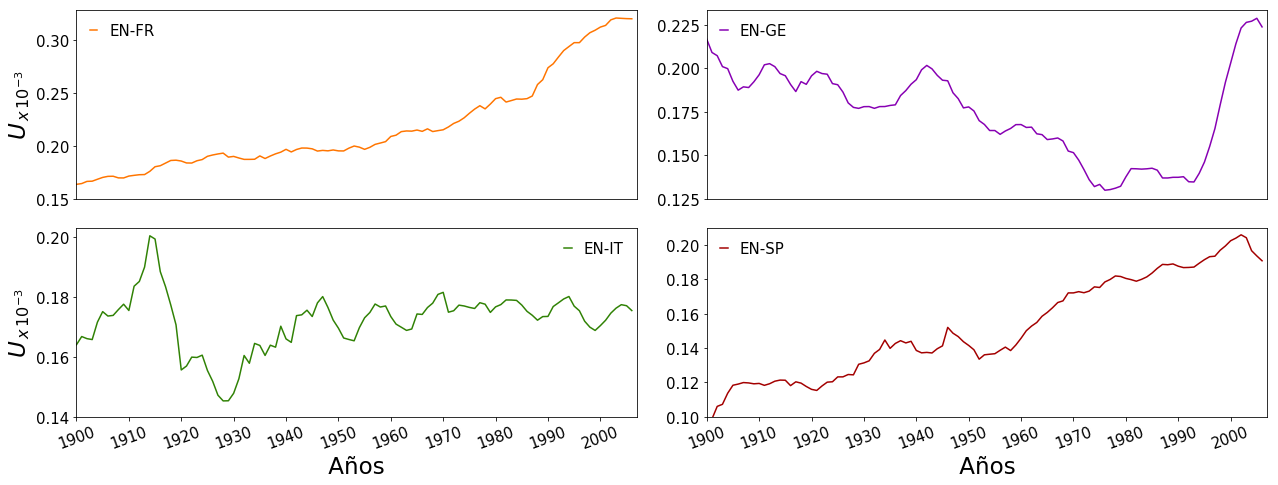
\includegraphics[scale=.33]{UO1_EN.png}
	\caption{El uso del inglés en los demás idiomas. El mayor aumento en el uso del inglés se dio en el alemán, a razón de 0.0054~ppa  entre 1990 y 2003, después en el francés con 0.0018~ppa entre 1945 y 2009, y en el español con 0.0012~ppa entre 1950 y 2000. El uso del inglés en el el italiano, disminuyó a razón de -0.0013~ppa entre 1910 y 1930.}
	\label{fig.UO_EN}
\end{figure} 

De la figura~\ref{fig.UO_EN} se puede ver que el uso del inglés en el francés, en el español y en el italiano aumentó después de 1930, mientras que en el alemán fue posterior a 1990.  La causa de estos aumentos, se asocia con el surgimiento de los Estados Unidos como una potencia mundial después de finalizar la Segunda Guerra Mundial,  al  imponer  su modelo económico e impulsar el desarrollo de la ciencia y la tecnología durante la Guerra Fría.

Los préstamos acumulados que son comunes en los cuatro receptores y que aumentan su influencia, son de los campos semánticos de la economía y de la tecnología. Entre ellos están \textit{capital}, \textit{dollar}, \textit{invesment}, \textit{relations}, \textit{market}, \textit{company}, \textit{development}, \textit{financial},  \textit{institutions}, \textit{internet}, \textit{windows} y \textit{software}. Otros préstamos importantes son los apellidos de los presidentes de los Estados Unidos desde la Segunda Guerra Mundial. Todos ellos fueron relevantes durante el periodo en el cual gobernaron. 
\label{EN-D}

\begin{figure}[h!]
	\centering
	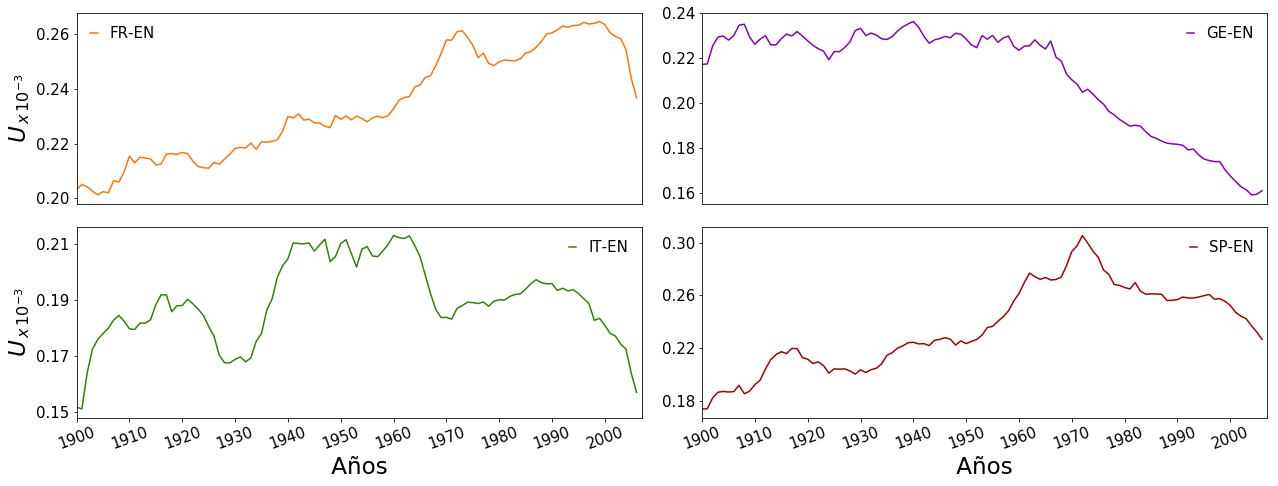
\includegraphics[scale=.33]{UR1_EN.png}
	\caption{El uso de los demás idiomas en el inglés. El idioma que más aumento su uso en el ingles fue el italiano, a razón de 0.003 ppa entre 1930 y 1940, seguido del español con 0.0016~ppa y del francés con 0.0008~ppa, ambos entre 1920 y 1970. El alemán disminuyó su uso en el inglés, a razón de -0.0015~ppa entre 1970 y 2009.}
	%Los idiomas que más aumentaron por cada año su uso en el inglés, son el español con 0.038 entre 1945 y 1970, el francés con 0.014 entre 1960 y 2006, y el italiano con 0.0019 entre 1930 y 1950.
	\label{fig.UR_EN}
\end{figure} 


De la figura~\ref{fig.UR_EN} se puede ver que después que durante la Segunda Guerra Mundial, los valores del uso del italiano y del alemán eran similares, alrededor de 0.22$\pm$0.01 La similitud se mantuvo hasta 1960, donde su uso en el inglés disminuyó, consecuencia de que Alemania e Italia perdieran la guerra.

Los préstamos acumulados que descendieron en rango son referentes al conflicto. Entre ellos \textit{berlin}, \textit{hitler} y \textit{lenin}, son del alemán,  mientras que \textit{mussolini} y \textit{regime} son del italiano. 

Por otra parte, el español y el francés aumentaron su uso en el inglés después de la Segunda Guerra Mundial, sin embargo  referente al francés, los préstamos que aumentan su influencia entre 1950 y 2000 son del campo semántico de la religión. Entre ellos están \textit{dieu}, \textit{eveque}, \textit{religion}, \textit{saint} y \textit{eglise}.

Con el español, las palabras que más influyeron en el aumento entre 1950 y 1970 son nombres de países latinoamericanos. En este periodo, algunos de ellos tuvieron alguna relación histórica con los Estados Unidos como \textit{mexico} y \textit{cuba}; mientras otros como \textit{chile}, \textit{peru} y \textit{argentina}, destacaron por tener crisis económicas y golpes de estado en la posguerra.  
\label{D-EN}


 
%Apoyado de la información de los préstamos nuevos, se puede confirmar que el inglés se ha beneficiado del crecimiento de los Estados Unidos para ser exportado a las demás lenguas y ser el idioma común para transmitir información.   

%Tras brevemente ver ambos conjuntos se infiere que el español ha logrado instaurarse en el inglés por la relevancia de estos países en las relaciones o conflictos que tuvieron en el siglo pasado y donde intervinieron países de habla inglesa, contrario  al francés que prevalece por las relaciones culturales y etimológicas que existen entre ambas lenguas.


% }}}
\subsection{Francés} % {{{

\begin{figure}[h!]
	\centering
	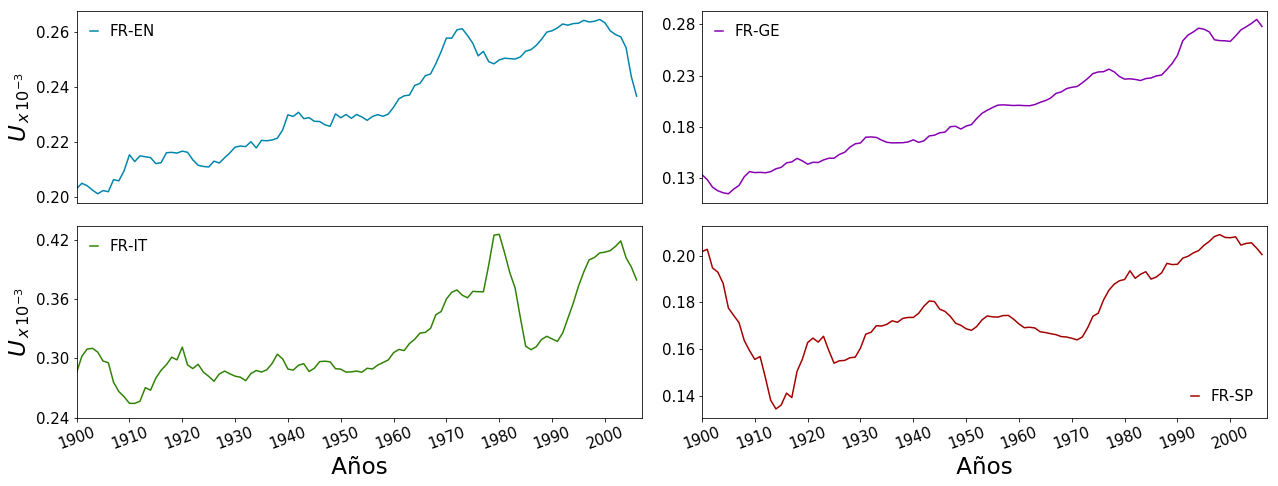
\includegraphics[scale=.33]{UO1_FR.png}
	\caption{El uso del francés en los demás idiomas. El mayor aumento en el uso del francés se dio en en el italiano, a razón de 0.0031 ppa entre 1950 y 1970, después en el español con 0.0015~ppa entre 1970 y 1995, en el alemán con 0.0013~ppa entre 1900 y 2009 y en el inglés con 0.008~ppa entre 1920 y 1970.}
	\label{fig.UO_FR}
\end{figure}

De la figura~\ref{fig.UO_FR} se puede ver que durante todo el siglo XX, el italiano es el idioma donde el francés es más usado, a pesar de que el inglés tenga más préstamos acumulados del francés, de acuerdo a la tabla~\ref{tab.cantidad_acumulados}. 


A pesar de que entre 1910 y 1940 ocurriesen las dos Guerras Mundiales, y tanto Francia como Italia participaran en ellas,  los préstamos que aumentaron su influencia en este periodo no son referentes al conflicto, estos son del campo semántico de la industria vitivinícola, una industria común en Francia e Italia. Entre los préstamos se encuentran \textit{raisins}, \textit{vin}, \textit{vignoble} y \textit{recolte}. 

Las palabras involucradas en el aumento del uso del francés en el alemán, en el inglés y en el español, entre 1940 y el 2000, son de los campos semánticos de la religión y de la Revolución Francesa. De la religión se encuentran \textit{saint}, \textit{eglise} y \textit{dime}; mientras que \textit{reine}, \textit{forteresse}, \textit{napoleon}, \textit{guerre}, \textit{imperiale}, \textit{bastille}, \textit{royals} y \textit{bourgeois} son de la Revolución Francesa. 
\label{FR-D}


\begin{figure}[h!]
	\centering
	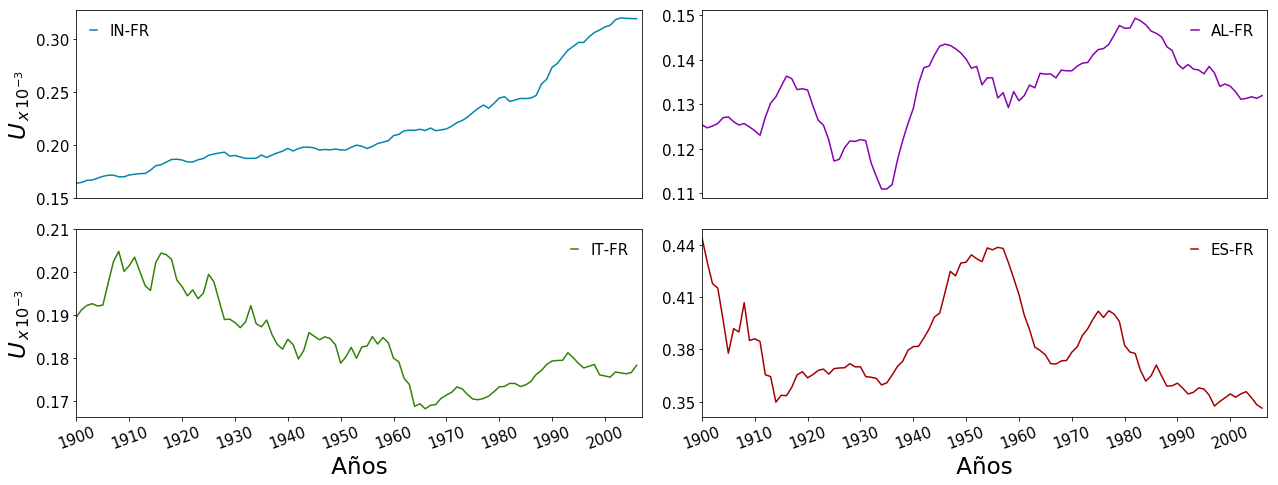
\includegraphics[scale=.33]{UR1_FR.png}
	\caption{El uso de los demás idiomas en el francés. El idioma que más aumentó su uso en el francés fue el español, a razón de  0.0026 ppa entre 1930 y 1955, seguido del inglés con 0.0018~ppa entre 1945 y 2009, y del alemán con 0.0014~ppa entre 1930 y 1945. El italiano  disminuyó su uso en el francés, a razón de -0.0002~ppa entre 1905 y 1960.}
	\label{fig.UR_FR}
\end{figure}
		
De acuerdo a la tabla \ref{tab.cantidad_acumulados},  el español es el tercer idioma que más prestamos acumulados tiene en el francés, sin embargo, durante todo el siglo XX, el español como se puede ver en la figura~\ref{fig.UR_FR}, fue el idioma con el mayor uso en el francés.

Los prestamos involucrados en el aumento del uso del inglés en el francés son de los campos semánticos de la economía y la tecnológica. Estos términos, ya se han mencionado en los préstamos acumulados del inglés en los demás idiomas (página~\pageref{EN-D}).
	
La característica común de los prestamos acumulados del español en el francés que descendieron en rango durante el siglo XX, es que son palabras con etimología grecolatina,  como \textit{principe}, \textit{servicios}, \textit{comite}, \textit{canal}, \textit{tribunal}, \textit{proceso}, \textit{central} y \textit{normal}. 
\label{D-FR}



% }}}
\subsection{Alemán} % {{{

\begin{figure}[h!]
	\centering
	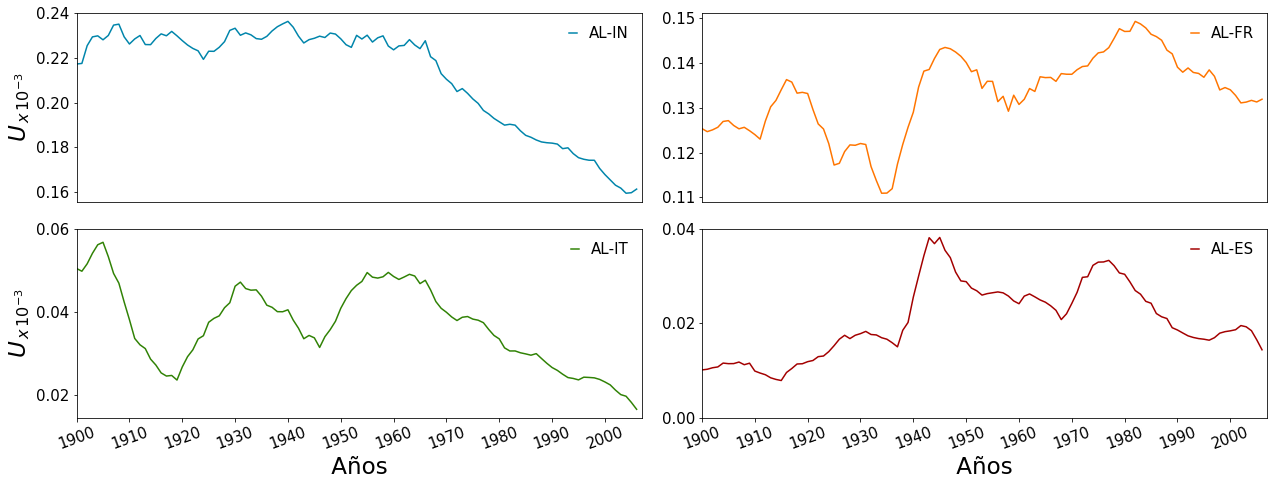
\includegraphics[scale=.33]{UO1_GE.png}
	\caption{El uso del alemán en los demás idiomas. El mayor aumento en el uso del alemán se dio en el español, a razón de 0.0021 ppa entre 1935 y 1945, y después en el francés con 0.0014~ppa entre 1930 y 1945.  Entre 1960 y 2009, el uso del alemán disminuyó  a razón de -0.0015~ppa en el inglés, y -0.0006~ppa en el italiano.}
	\label{fig.UO_GE}

\end{figure}



De la figura~\ref{fig.UO_GE} se puede ver que el uso del alemán en el
inglés y en el italiano disminuyó a partir de 1960. Entre los préstamos del alemán que perdieron influencia en ambos idiomas a partir de este año, están \textit{berlin}, \textit{marx}, \textit{hitler}, \textit{lenin}, \textit{testen} y \textit{reich}, palabras del campo semántico de la Segunda Guerra Mundial. 

En el francés y en el español, las palabras que aumentaron su influencia entre 1930 y 1980,  son los apellidos personajes germano parlantes que destacaron en algún área académica. Entre ellos están \textit{marx}, \textit{Freud}, \textit{heidegger}, \textit{nietzsche}, \textit{hegel}, \textit{engels} y \textit{mozart}.

\label{GE-D}


\begin{figure}[h!]
	\centering
	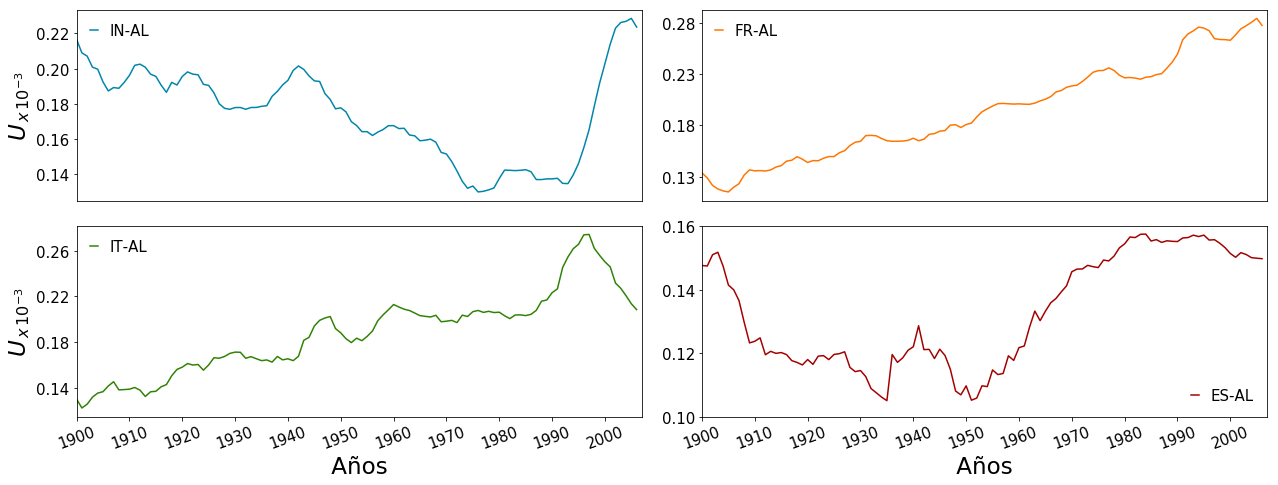
\includegraphics[scale=.33]{UR1_GE.png}
	\caption{El uso de los demás idiomas en el alemán. El idioma que más aumentó su uso en el alemán fue el inglés, a razón de 0.0054 ppa  entre 1990 y 2003, seguido del español con 0.0014~ppa entre 1950 y 1980, el francés con 0.0013~ppa entre 1900 y 2009, y el italiano con 0.0010~ppa entre 1900 y 1995.}
	\label{fig.UR_GE}
\end{figure}

De la figura~\ref{fig.UR_GE} se puede ver que el español durante la primera mitad de siglo, fue el idioma que menor uso tuvo en el alemán, además coincide con ser el idioma que menos préstamos acumulados tiene en el alemán (tabla~\ref{tab.cantidad_acumulados}). Palabras del campo semántico de la medicina como \textit{virus}, \textit{anemia}, son las que disminuyeron su influencia en el alemán. 

El uso los demás idiomas en el alemán, aumentó debido a palabras de diferentes campos semánticos, la  economía y la tecnología  por parte del inglés (página~\pageref{EN-D}); la religión y la Revolución Francesa por parte del francés (página~\pageref{FR-D}); mientras que del italiano 
\textit{liberale}, \textit{sociale}, \textit{mussolini} y  \textit{regime} 
son de la política y  de la Segunda Guerra Mundial.

\label{D-GE}

% }}}
\subsection{Italiano} % {{{

\begin{figure}[h!]
	\centering
	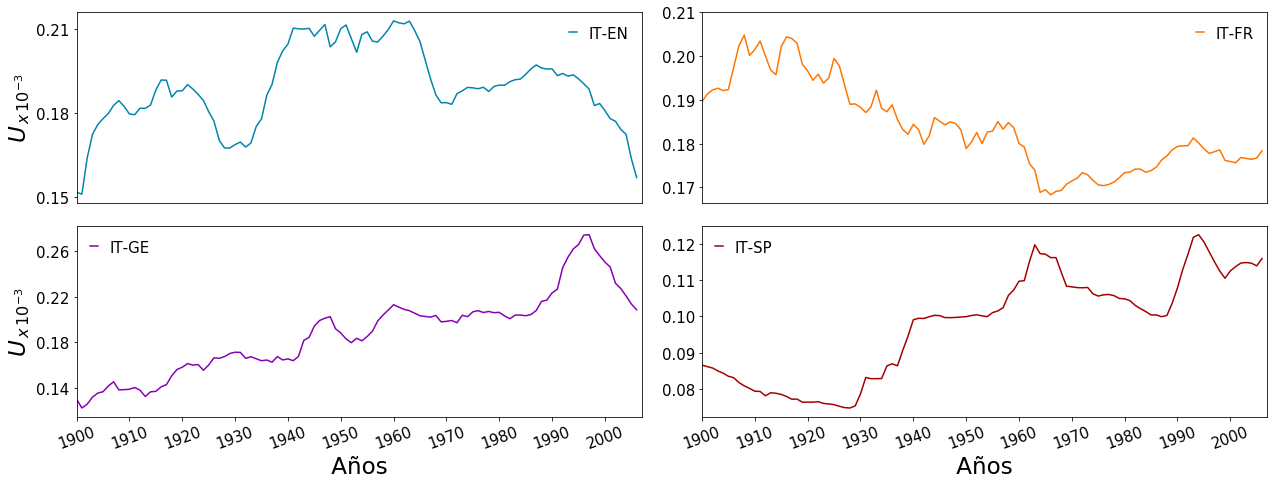
\includegraphics[scale=.33]{UO1_IT.png}
	\caption{El uso del italiano en los demás idiomas. El mayor aumento en el uso del italiano se dio en el inglés, a razón de 0.0035 ppa entre 1930 y 1940, después en español con 0.0011~ppa entre 1930 y 1960, y en alemán con 0.0010~ppa entre 1900 y 1995. El uso del italiano en el francés, disminuyó a razón de -0.0002~ppa  entre 1905 y 1960.}
	\label{fig.UO_IT}
\end{figure}
	
Los préstamos del italiano que se relacionaron con campos semánticos, son \textit{mussolini}, \textit{fascismo}, \textit{battaglia} y \textit{regime} con la guerra; \textit{sociale},  y \textit{liberale} con la politica;  y \textit{santo}, \textit{suora} y \textit{cattedrale} con la religión.

Estos préstamos, como se puede ver en la figura~\ref{fig.UO_IT}, aumentaron el uso del italiano en el inglés entre 1930 y 1940, en el francés entre 1960 y 2009, en el alemán entre 1900 y 1995, y en el español entre 1930 y 1960.
\label{IT-D}


\begin{figure}[h!]
	\centering
	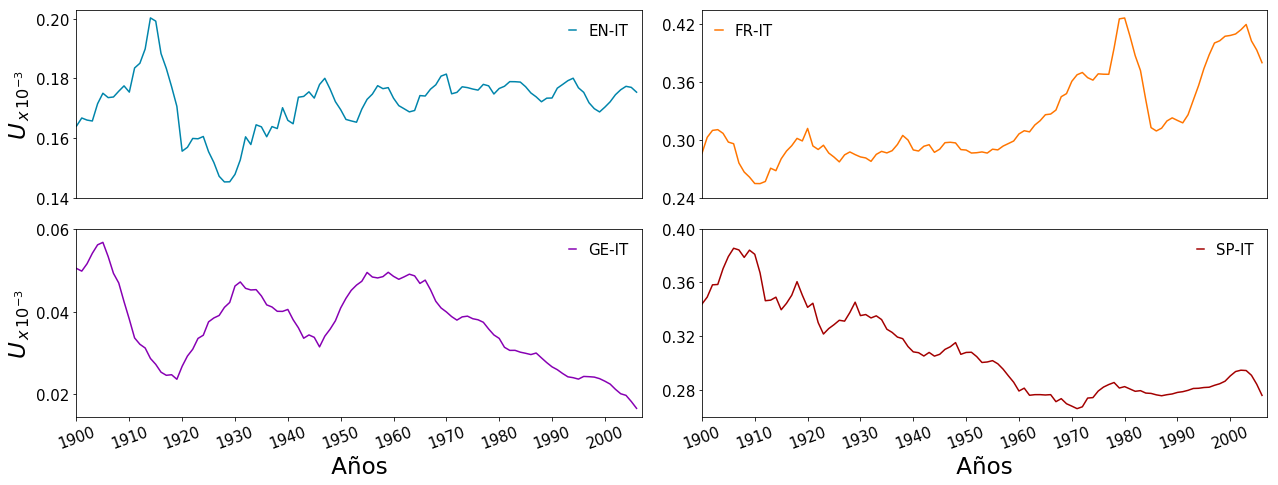
\includegraphics[scale=.33]{UR1_IT.png}
	\caption{El uso de los demás idiomas en el italiano. El idioma que más 
	disminuyó su uso en el italiano fue el español, a razón de -0.0017 ppa entre 1905 y 1970, seguido del inglés con -0.0013~ppa entre 1910 y 1930, y del alemán con -0.0006~ppa entre 1960 y 2009. El francés aumentó su uso en el italiano, a razón de 0.0031~ppa entre 1950 y 1975.}
	\label{fig.UR_IT}
\end{figure}

De la figura~\ref{fig.UR_IT} se puede ver que el francés desde 1930, es el idioma con el mayor uso en el italiano, a pesar de que el español tenga más préstamos acumulados en el italiano, de acuerdo a la tabla~\ref{tab.cantidad_acumulados}. Los préstamos del español que disminuyeron su influencia son referentes a Latinoamérica, entre ellos  \textit{argentina}, \textit{buenos}, \textit{aires}, \textit{america} y \textit{latina}.

Los préstamos de los demás idiomas en el italiano, son de la economía y tecnología por parte del inglés (página~\pageref{EN-D}), la industria vitivinícola por parte del francés (página~\pageref{FR-D}), y de la Segunda Guerra Mundial por parte del alemán (página~\pageref{GE-D}).

\label{DE-IT}



% }}}
\subsection{Español} % {{{
\begin{figure}[h!] % {{{
	\centering
	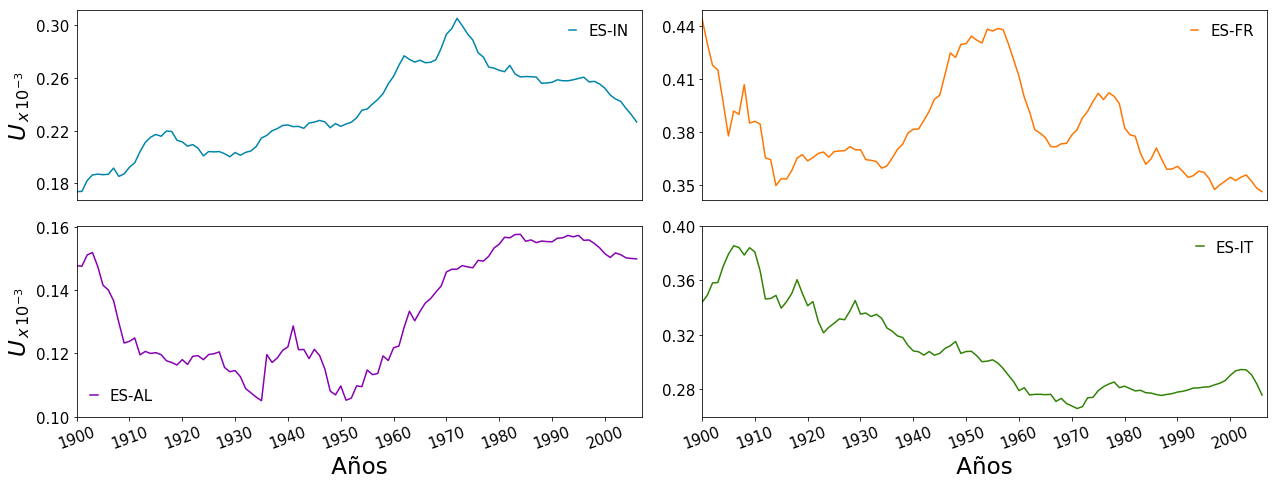
\includegraphics[scale=.33]{UO1_SP.png}
	\caption{El uso del español en los demás idiomas. El mayor aumento en el uso del español se dio en el francés, a razón de 0.0026 ppa entre 1930 y 1955, después en el inglés con 0.016~ppa entre 1920 y 1970,  y en el alemán con 0.0014~ppa entre 1950 y 1980. El uso del español en el italiano, disminuyó a razón de -0.0017~ppa entre 1905 y 1970.}
	\label{fig.UO_SP}
	
\end{figure} % }}}

Entre los préstamos del español en el inglés, se encuentran nombres de 
estados de los Estados Unidos con gran población hispanohablante como \textit{california} y \textit{florida};  y también nombres de países y ciudades en Latinoamérica como \textit{mexico}, \textit{panama}, \textit{chile}, \textit{cuba}, \textit{peru}, \textit{colombia}, \textit{argentina}, \textit{buenos} y \text{aires}. Estas palabras reflejan la relación cultural entre Latinoamérica y Los Estados Unidos, además son las que aumentan más su influencia 


De la figura~\ref{fig.UO_SP}, el aumento del uso del español en el inglés entre 1920 y 1970 se debe a la relación cultural e histórica entre países de Latinoamérica con los Estados Unidos. Entre estos años, las palabras que aumentaron su influencia son  nombres de estados de los Estados Unidos con gran población hispanohablante como \textit{california} y \textit{florida};  y nombres de países y ciudades en Latinoamérica como \textit{mexico}, \textit{panama}, \textit{chile}, \textit{cuba}, \textit{peru}, \textit{colombia}, \textit{argentina}, \textit{buenos} y \textit{aires}.

Los préstamos del español que se encuentran presentes en todos los idiomas, son términos de la medicina. Entre ellas están \textit{terapia}, \textit{anemia}, \textit{lepra}, \textit{tumor}, \textit{syphilis}, \textit{virus} y \textit{renal}.
 
\label{SP-D}

		
\begin{figure}[h!] % {{{
	\centering
	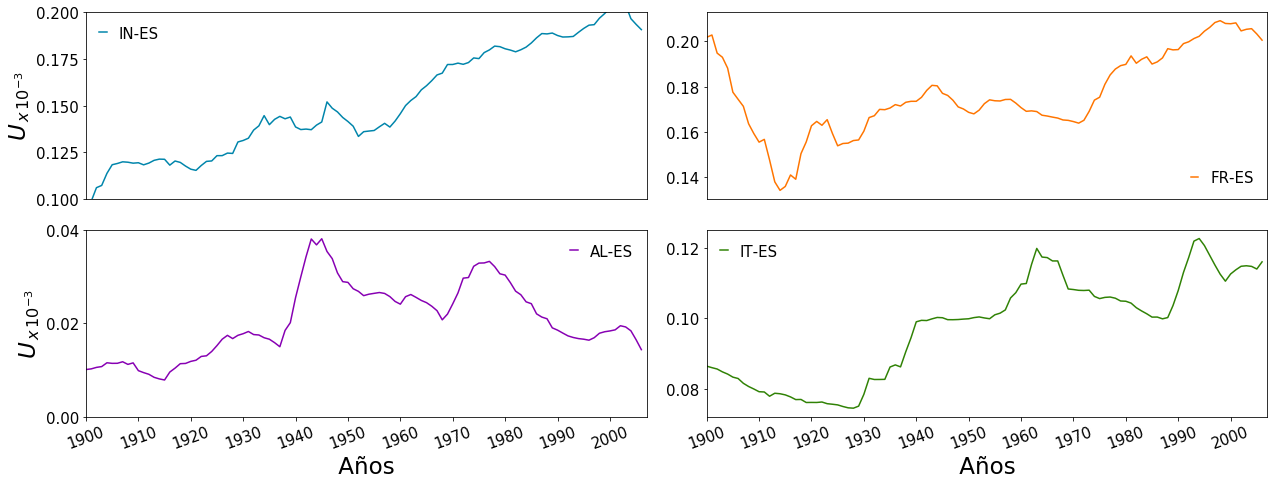
\includegraphics[scale=.33]{UR1_SP.png}
	\caption{El uso de los demás idiomas en el español. El idioma que más aumentó su uso en el español fue el alemán, a razón de 0.0021 ppa entre 1935 y 1945, seguido del francés con 0.0015~ppa entre 1970 y 1995,  del inglés con 0.0012~ppa entre 1950 y 2000, y del italiano con 0.0011~ppa entre 1930 y 1960.}
	\label{fig.UR_SP}
\end{figure}

De la figura~\ref{fig.UR_SP} se puede ver que el inglés y el francés, son los idiomas que mayor uso tienen en el español, pese a que entre ambos, la cantidad de préstamos acumulados que tienen en el español sea dos tercios de la que tiene el italiano, de acuerdo a la tabla~\ref{tab.cantidad_acumulados}.

%el italiano, tenga el doble de préstamos acumulados en el español, que el inglés y el francés juntos, de acuerdo a la tabla~\ref{tab.cantidad_acumulados}.  


Los préstamos de los demás idiomas en el español, son de la economía y tecnología por parte del inglés (página~\pageref{EN-D}), la Revolución Francesa y la religión por parte del francés (página~\pageref{FR-D}), apellidos de personajes germano parlantes que destacaron en algún área académica  por parte del alemán (página~\pageref{GE-D}), y la guerra, la política y la religión por parte del italiano (página~\pageref{IT-D}).  


%En las discusiones anteriores se han mencionado,  los préstamos que modifican su influencia en el español, disminuyendo los del alemán  en el campo semántico de la guerra (página~\pageref{GE-D}), y aumentando los del inglés en la economía y la tecnología (página~\pageref{EN-D}),  los del francés en la revolución francesa y en la religión (página~\pageref{FR-D}),  y los del italiano en la religión, la política y la guerra (página~\pageref{IT-D}).

\label{D-SP}




% }}}
% }}}
% }}}
\section{Resultados generales} % {{{


El determinar la influencia entre idiomas a través del uso permitió ver  que el idioma más usado no es siempre el que tiene la mayor cantidad de préstamos acumulados.  Un mayor uso significará que los préstamos acumulados tienen rangos más bajos (frecuencias altas) en el idioma receptor.

El uso también mostró que en los periodos de tiempo donde el uso de un idioma en otro aumenta o disminuye, están involucradas palabras de campos semánticos, que también aumentan o disminuyen su influencia.  Además, se corroboran las conclusiones de los préstamos nuevos, donde en cada idioma influyen más ciertos campos semánticos, en el inglés la economía, la tecnología y la política; en el francés la religión, la Revolución Francesa y la industria vitivinícola; en el alemán la guerra y los apellidos de personajes germano parlantes que destacaron en algún área académica; en el italiano la guerra, la política y la religión; y en el español la medicina y la cultura de los países Latinoamericanos.

Respecto a las listas de los préstamos acumulados de cada pareja de idiomas, se observo que los primeros tres rangos en cada lista están usualmente ocupados por las mismas palabras. Como las palabras que ascienden o descienden en rango son las que modifican su influencia, entonces estás palabras deben tener rangos más altos que $k=3$. Se discutirá en el capítulo 6 la forma en que varían las palabras que tienen un mismo rango $k$.



Los resultados del uso entre idiomas por el momento son limitados, sólo es posible explicar por qué varia el uso de un idioma en otro,  a través de las palabras que están involucradas. No es posible predecir como se comportará el uso en el futuro, ni que palabras intervendrán. No obstante, se pueden obtener mejores resultados y explicaciones si se comparará el uso con datos específicos de los países, como lo pueden ser el producto interno bruto, la alfabetización, la mortalidad o  las migraciones de personas, entre otros.

%Se destaca a los eventos como una característica que modifica el uso entre idiomas, sin embargo se podría obtener una mejor conclusión, si se comparará el uso con datos específicos de los países, como lo pueden ser, el producto interno bruto, la alfabetización, la mortalidad, las migraciones de personas, entre otros.

 

%Una mejor información de como los eventos alteran a los idiomas se podría extraer si se compararán las características de los prestamos con  datos de los países de alguna habla como lo pueden ser  el crecimiento economizo, el producto interno bruto, la alfabetización, la mortalidad, las migraciones de personas, entre otros.

%En todo el siglo XX y la primer década del XXI, el inglés y el alemán han sido los idiomas más cambiantes en los papeles de origen y receptor. En cualquier combinación con otro idioma el uso ha sido alterado en alguna época. 
%El inglés al ser el que más creció en tres idiomas (francés, alemán y español), complementando los resultados del capitulo anterior, al ser el idioma que más palabras nuevas exportó.  El alemán como el receptor donde los diferentes orígenes aumentaron su usó tras la segunda guerra mundial; el uso ha sido semejante a los préstamos nuevos, ha sido el receptor que más recibió. 
%Ambos análisis se complementan,  el idioma más influyente ha aportado más palabras nuevas y aquellas que se van acumulando resultan las de mayor incremento en el uso. El idioma más influenciado recibió la mayor cantidad de palabras nuevas y el uso que han tenido los demás ha sido también el del mayor incremento. 

 




% }}}

